% Dokumentenkopf ---------------------------------------------------------------
%   Diese Vorlage basiert auf "scrreprt" aus dem koma-script.
% ------------------------------------------------------------------------------
\documentclass[
    12pt, % Schriftgr��e
    DIV10,
    ngerman, % f�r Umlaute, Silbentrennung etc.
    a4paper, % Papierformat
    oneside, % einseitiges Dokument
    titlepage, % es wird eine Titelseite verwendet
    parskip=half, % Abstand zwischen Abs�tzen (halbe Zeile)
    headings=normal, % Gr��e der �berschriften verkleinern
    listof=totoc, % Verzeichnisse im Inhaltsverzeichnis auff�hren
    bibliography=totoc, % Literaturverzeichnis im Inhaltsverzeichnis auff�hren
    index=totoc, % Index im Inhaltsverzeichnis auff�hren
    captions=tableheading, % Beschriftung von Tabellen unterhalb ausgeben
    final % Status des Dokuments (final/draft)
]{scrreprt}

% ben�tigte Packages -----------------------------------------------------------
%   LaTeX-Packages, die ben�tigt werden, sind in die Datei Packages.tex
%   "ausgelagert", um diese Vorlage m�glichst �bersichtlich zu halten.
% ------------------------------------------------------------------------------
% Anpassung des Seitenlayouts --------------------------------------------------
%   siehe Seitenstil.tex
% ------------------------------------------------------------------------------
\usepackage[
    automark, % Kapitelangaben in Kopfzeile automatisch erstellen
    headsepline, % Trennlinie unter Kopfzeile
    ilines % Trennlinie linksb�ndig ausrichten
]{scrpage2}

% Anpassung an Landessprache ---------------------------------------------------
\usepackage[ngerman]{babel}

% Umlaute ----------------------------------------------------------------------
%   Umlaute/Sonderzeichen wie ���� direkt im Quelltext verwenden (CodePage).
%   Erlaubt automatische Trennung von Worten mit Umlauten.
% ------------------------------------------------------------------------------
\usepackage[latin1]{inputenc}
\usepackage[T1]{fontenc}
\usepackage{textcomp} % Euro-Zeichen etc.

% Schrift ----------------------------------------------------------------------
\usepackage{lmodern} % bessere Fonts
\usepackage{relsize} % Schriftgr��e relativ festlegen
\usepackage{icomma} % Abst�nde vor den Kommas sind kleiner

% Grafiken ---------------------------------------------------------------------
% Einbinden von JPG-Grafiken erm�glichen
%\usepackage[dvips,final]{graphicx}
\usepackage{graphicx}
% hier liegen die Bilder des Dokuments
\graphicspath{{Bilder/}}

% Bibliothek f�r Tabellen
\usepackage{caption}
\usepackage{booktabs}
\usepackage{multirow}

% Befehle aus AMSTeX f�r mathematische Symbole z.B. \boldsymbol \mathbb --------
\usepackage{amsmath,amsfonts}

% physikalische Einheiten ------------------------------------------------------
\usepackage{siunitx}

% Schaltkreise zeichnen --------------------------------------------------------
\usepackage{tikz}
\usepackage[siunitx]{circuitikz}
\usetikzlibrary{arrows,shapes,calc,positioning}

% f�r Index-Ausgabe mit \printindex --------------------------------------------
\usepackage{makeidx}

% Einfache Definition der Zeilenabst�nde und Seitenr�nder etc. -----------------
\usepackage{setspace}
\usepackage{geometry}

% Symbolverzeichnis ------------------------------------------------------------
%   Symbolverzeichnisse bequem erstellen. Beruht auf MakeIndex:
%     makeindex.exe %Name%.nlo -s nomencl.ist -o %Name%.nls
%   erzeugt dann das Verzeichnis. Dieser Befehl kann z.B. im TeXnicCenter
%   als Postprozessor eingetragen werden, damit er nicht st�ndig manuell
%   ausgef�hrt werden muss.
%   Die Definitionen sind ausgegliedert in die Datei "Glossar.tex".
% ------------------------------------------------------------------------------
\usepackage[intoc]{nomencl}
\let\abbrev\nomenclature
\renewcommand{\nomname}{Abk�rzungsverzeichnis}
\setlength{\nomlabelwidth}{.25\hsize}
\renewcommand{\nomlabel}[1]{#1 \dotfill}
\setlength{\nomitemsep}{-\parsep}

% zum Umflie�en von Bildern ----------------------------------------------------
\usepackage{floatflt}

% zum Einbinden von Programmcode -----------------------------------------------
\usepackage{listings}
\usepackage{xcolor} 
\definecolor{hellgelb}{rgb}{1,1,0.9}
\definecolor{colKeys}{rgb}{0,0,1}
\definecolor{colIdentifier}{rgb}{0,0,0}
\definecolor{colComments}{rgb}{1,0,0}
\definecolor{colString}{rgb}{0,0.5,0}
\lstset{
    float=hbp,
    basicstyle=\ttfamily\color{black}\small\smaller,
    identifierstyle=\color{colIdentifier},
    keywordstyle=\color{colKeys},
    stringstyle=\color{colString},
    commentstyle=\color{colComments},
    columns=flexible,
    tabsize=2,
    frame=single,
    extendedchars=true,
    showspaces=false,
    showstringspaces=false,
    numbers=left,
    numberstyle=\tiny,
    breaklines=true,
    backgroundcolor=\color{hellgelb},
    breakautoindent=true
}

% URL verlinken, lange URLs umbrechen etc. -------------------------------------
\usepackage{url}

% wichtig f�r korrekte Zitierweise ---------------------------------------------
% \usepackage[square]{natbib}
\usepackage{natbib}

% PDF-Optionen -----------------------------------------------------------------
\usepackage[
    bookmarks,
    bookmarksopen=true,
    colorlinks=true,
% diese Farbdefinitionen zeichnen Links im PDF farblich aus
    linkcolor=red, % einfache interne Verkn�pfungen
    anchorcolor=black,% Ankertext
    citecolor=blue, % Verweise auf Literaturverzeichniseintr�ge im Text
    filecolor=magenta, % Verkn�pfungen, die lokale Dateien �ffnen
    menucolor=red, % Acrobat-Men�punkte
    urlcolor=cyan, 
% diese Farbdefinitionen sollten f�r den Druck verwendet werden (alles schwarz)
    %linkcolor=black, % einfache interne Verkn�pfungen
    %anchorcolor=black, % Ankertext
    %citecolor=black, % Verweise auf Literaturverzeichniseintr�ge im Text
    %filecolor=black, % Verkn�pfungen, die lokale Dateien �ffnen
    %menucolor=black, % Acrobat-Men�punkte
    %urlcolor=black, 
    backref,
    plainpages=false, % zur korrekten Erstellung der Bookmarks
    pdfpagelabels, % zur korrekten Erstellung der Bookmarks
    hypertexnames=false, % zur korrekten Erstellung der Bookmarks
    linktocpage % Seitenzahlen anstatt Text im Inhaltsverzeichnis verlinken
]{hyperref}

% Befehle, die Umlaute ausgeben, f�hren zu Fehlern, wenn sie hyperref als Optionen �bergeben werden
% \hypersetup{
% pdftitle={\titel \untertitel},
% pdfauthor={\autor},
% pdfcreator={\autor},
% pdfsubject={\titel \untertitel},
% pdfkeywords={\titel \untertitel},
%}

% fortlaufendes Durchnummerieren der Fu�noten ----------------------------------
\usepackage{chngcntr}

% Acronympaket f�r Abk�rzungen ----------------------------------
\usepackage{acronym}
%\usepackage[printonlyused,withpage]{acronym}

% f�r lange Tabellen -----------------------------------------------------------
\usepackage{longtable}
\usepackage{array}
\usepackage{ragged2e}
\usepackage{lscape}

% Spaltendefinition rechtsb�ndig mit definierter Breite ------------------------
\newcolumntype{w}[1]{>{\raggedleft\hspace{0pt}}p{#1}}

% Formatierung von Listen �ndern -----------------------------------------------
\usepackage{paralist}

% bei der Definition eigener Befehle ben�tigt
\usepackage{ifthen}

% definiert u.a. die Befehle \todo und \listoftodos
\usepackage{todonotes}

% sorgt daf�r, dass Leerzeichen hinter parameterlosen Makros nicht als Makroendezeichen interpretiert werden
\usepackage{xspace}


% Erstellung eines Index und Abk�rzungsverzeichnisses aktivieren ---------------
\makeindex
\makenomenclature

% Das eigentliche Dokument -----------------------------------------------------
%   Der eigentliche Inhalt des Dokuments beginnt hier. Die einzelnen Seiten
%   und Kapitel werden in eigene Dateien ausgelagert und hier nur inkludiert.
% ------------------------------------------------------------------------------
\begin{document}

\chapter{Forward and inverse kinematics}

\section{UR5}
Universal Robots (UR1,-3,-5,-10) are multifunctional, flexible robots that can be used for various tasks. 
The number stands for the working load and therefore also the size of the robot. These robots 
are place saving and can be easily reprogrammed for new requirements. \\

ref1 \\

The URs consist out of six rotational joints and seven fixed links. Therefore there are eight different
constellations of joint angles to reach a determined end-effector position. That means that for given joint parameters we can calculate one unique position, but for a given position there are eight different sets of angles. These eight constellations can be described as lefty/righty, up/down and flip/noflip. With lefty/righty we can distinguish between the second joint being on the right or left
side of the imaginary plane going through the origin of the coordinate system of the first joint. This distinction makes sence if the coordinate system of the second joints has an offset according to the coordinate system of the first joint.  Up/down describes the relation between the coordinate systems of the third and the fourth joint. If the fourth joint remains in the same position, the third joint can 
be below or above it. Therefore we distinguish between up and down. Finally flip/noflip describes
the wrist (5th joint) being flipped or not, meaning rotated by $\phi$ or $\phi$ + 180$^\circ$. 

\begin{minipage}{0.64\textwidth}	
		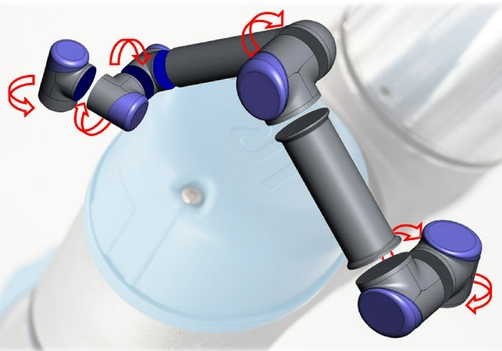
\includegraphics[width=\textwidth]{UR_joints}			
		\captionof{figure}{Joints of the UR, ref2}
\end{minipage}
\begin{minipage}{0.34\textwidth}
		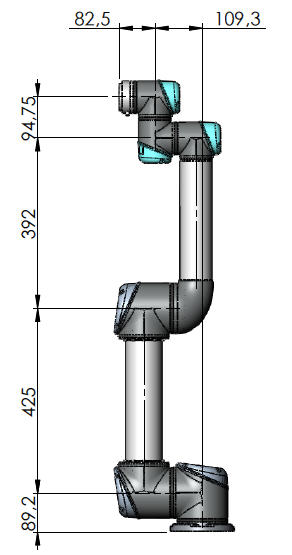
\includegraphics[width=\textwidth]{UR_dimensions}	
		\captionof{figure}{Dimensions of the UR, ref3}		
\end{minipage}

	%\begin{figure}[htbp]
		%\centering 
		%\captionsetup{format=plain}
			%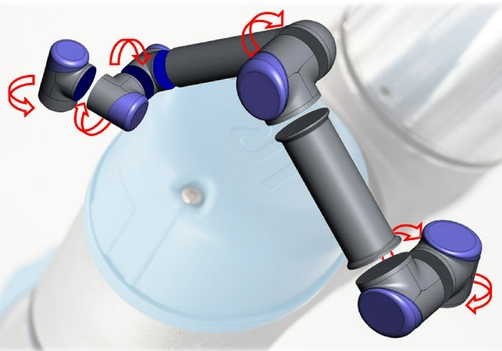
\includegraphics[width=1\textwidth]{UR_joints.jpg}		
				%\caption{Joints of the UR} 
				%\label{URJoints} 
	%\end{figure}

\section{Forward kinematics}
The forward kinematics of this kind of robot can be calculated easily with the Denavit-Hartenberg-procedure if the parameters are known. Denavit-Hartenberg-parameters describe the relation between two coordinate systems with a maximum of four different parameters: two rotation angles 
and two linear translations. These can be fixed or variable. In our case with six joints we have seven coordinate systems and six transfomations. Coordinate system zero is not attached to any of the joints and is used as the reference frame. \\

\section{Backward kinematics}
The backward kinematics has been realised with the algorithm of paper 

ref4 \\
 
Its starting point is the desired pose that we want to move our robot to. 
With this pose and the given Denavit-Hartenberg-parameters we calculate intermediate
poses from which the six angles can be found step by step. Previously calculated angles can furthermore be used to calculate the next ones. Since there are different angles possible to reach the same pose, it is important to name the current angle that is being used to calculate the next one. Lefty/righty, up/down and flip/noflip are current names. In case that one angle has two solutions the current solution exist with its particular name so
that the distinction between different possibilities is made. \\

The implemented algorithm works as follows:

\begin{itemize}
	\item Calculate eight max possible angle configurations that lead to the desired pose 
	\item Check if the pose is possible with the robots dimensions and/or the given maximal joint changes
	\item Calculate the $\pm$ 360$^\circ$-versions of the found angles since the robot might be able 
	to move in the range of $\pm$ 360$^\circ$ and get eight new possibilities
	\item Choose one angle set of the 16 sets with the minimal angle sum with respect to the initial angles
\end{itemize}
\chapter{Handy-Eye-calibration}

The hand-eye-calibration is a current procedure to determine unknown rigid transformations, e.g. transformations between the end-effector and a tool attached to it or a transformation between the robot and the tracking system,
by taking measurements with the tracking device in different poses of the robot. For good precision and accuracy you need many different poses and they need to be linearly independant from each other. 

In this project the transformation between the robots end-effector and the coil had to be 
determined as well as the transformation between the robots base and the coordinate system of the tracking device. The coil needed to be placed in a certain translation and rotation with respect to the head of the imaginary patient therefore it was not enough to know only the end-effector coordinates that can be calculated by the direct kinematics. The hand-eye-calibration uses the closed loop of four rigid transformations. That means that we can express one transformation or a combination of two by means of the remained ones. Two of these transformations are fixed and the other two can vary. Figure \ref{handeye} shows the installation.

\begin{figure}[htbp]
	\centering 
	\captionsetup{format=plain}
		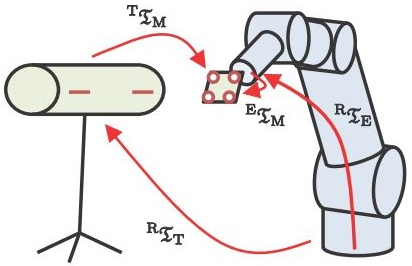
\includegraphics[width=0.8\textwidth]{handeye}		
			\caption{Hand-Eye-calibration setup} 
			\label{handeye} 
\end{figure}

\begin{equation}
	M = ^RT_E
\end{equation}

\begin{equation}
	X = ^ET_M
\end{equation}
	
\begin{equation}
	N = ^TT_M
\end{equation}
	
\begin{equation}
	Y = ^RT_T
\end{equation}

We are interested in the fixed ones $^E$T$_M$ and $^R$T$_T$ whereas the variable ones can be calculated or measured. We can write \\

\begin{equation}
	M \cdot X = Y \cdot N
\end{equation}

or 

\begin{equation}
	M_i \cdot X = N_i \cdot Y
\end{equation}

where index $i$ denotes one set of measurements. 

These equations can be rearranged and written as 

\begin{equation}
	A \cdot w = b
\end{equation}

where $A$ and $b$ contain manipulated values of $M_i$ and $N_i$ so that we can fill these matrices with 
actual measurement values to calculate $w$. After the calculation the solution vector $w$ contains the
24 not trivial values of $X$ and $Y$. The last step of the calibration is to orthonormalize $X$ and $Y$
since the calculation of $w$ provides independant values for the rotation and translation. 
If the translation can be taken as given, the vectors of the rotation matrix need to be orthonormal.  

ref5     
	
	
	


\end{document}
